\vspace*{-1mm}
In Chapter~\ref{Ch:2018_setup} the operational set up and the beam instrumentation used for the first measurements of noise induced emittance growth with $\CC$ and proton beams in the SPS were described. 


In this Chapter the experimental results are discussed. In particular, the measurements of the paramters of interest (described in Chapter~\ref{Ch:CC_noise_theory}, Eq.~\eqref{eq:dey_an} and Eq.~\eqref{eq:dey_pn}) and their analysis are presented. First, Section~\ref{sec:experimental_procedure_2018} explains the experimental procedure.  In Section~\ref{sec:CC_voltage_meas2018} the calibration of the $\CC$ voltage is displayed. Section~\ref{sec:noise_meas2018} elaborates on the injected noise and the acquistions of the power spectrum. Thereafter, in Section~\ref{sec:EmitGrowth_measurements} the measured emittance growth, which is the paramter of primary interest, is discussed. Furthermore, the measurements of the bunch length are examined in Section~\ref{sec:bunch_length_measurements_2018} while the intensity evolution is shown in Section~\ref{sec:intensity_measurements_2018} for completness. Section~\ref{sec:meas_2018_vs_theory} compares the measured emittance growth rates with the predictions of the theoretical model introduced in Chapter~\ref{Ch:CC_noise_theory}. Finally, Section~\ref{sec:MD2018_summary} summarizes the main experimental findings.



\section{Crab cavity voltage. Change beta functions of CC at the scripts, and the pay --> phase advance!!!}\label{sec:CC_voltage_meas2018}

As already mentioned above, the targetd $\CC$ voltage was 1\,MV. Nevetherless, beam based measurements with the HT monitor (post-processing in Section~\ref{sec:HT_info}) were carried out to validate this value. Unfortunately, only two measurements are available, which are displayed in Fig.~\ref{fig:VCC_MD5_2018}. The first measurement took place before the start of the first "coast", at $\sim$9:45 (left), while the second one took place at $\sim$13:50 between the first and the seond "coast" (right). 


% 1. locally PhD_projects/CC_MD_2021_summary/HT_monitor/2018_HT_monitor
% 2. lxplus: cernbox/2021/CC_MD_2021_summary/HT_monitor/2018_HT_monitor
\begin{figure}[!ht]
    \centering
    \begin{subfigure}[t]{0.45\textwidth}
        \centering
        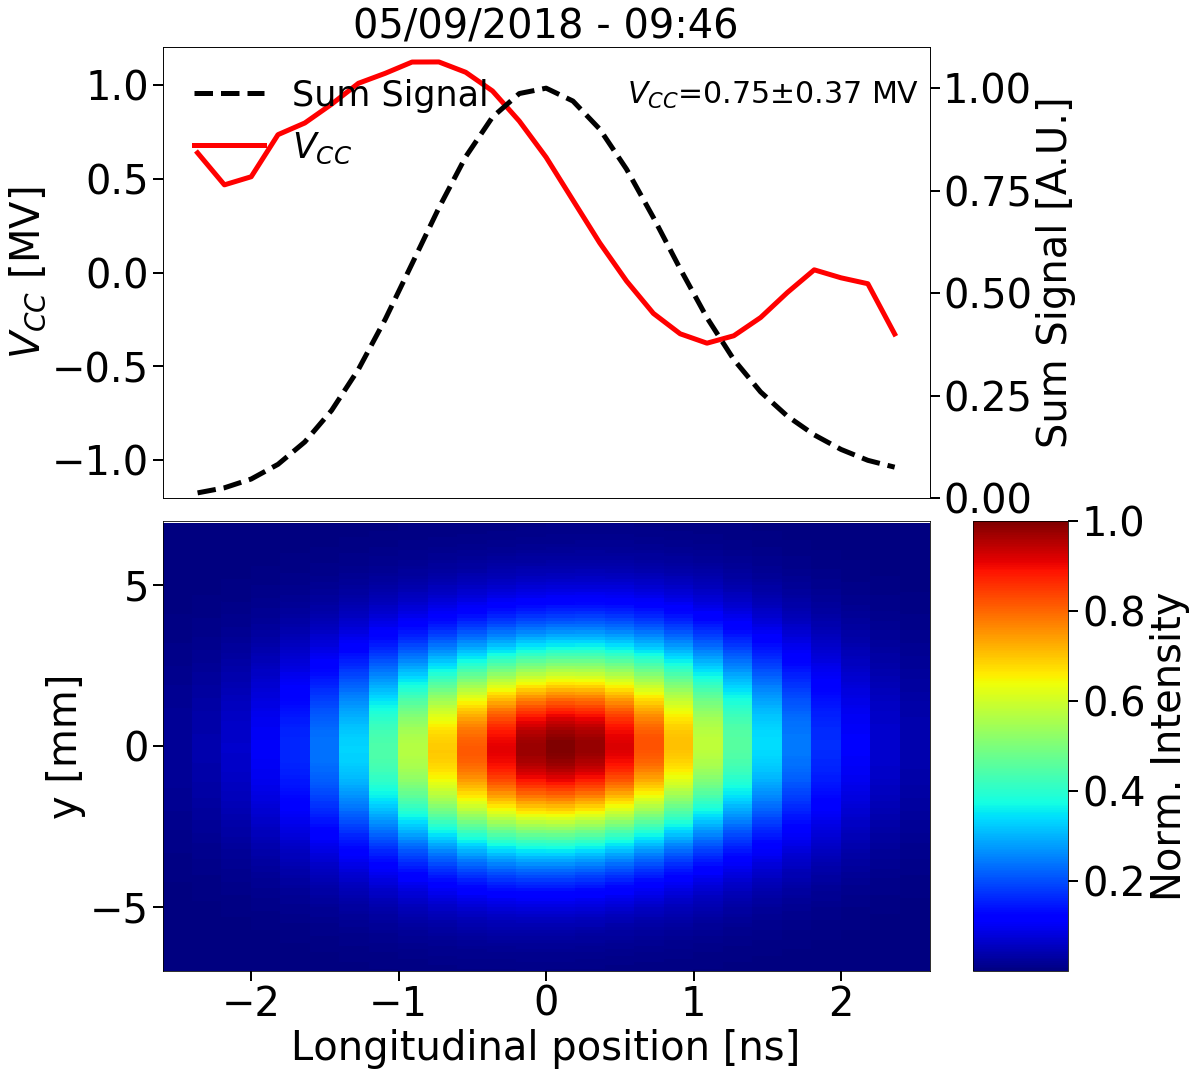
\includegraphics[width=1\textwidth]{images/Ch5/HT_crabVoltage__20180905_094640_crabbing_only.png}
        %\caption{$y=\sin(2 \pi f t),\ f=50$ Hz}
        %\label{fig:signal_and_DFT_example_a}
    \end{subfigure}
    \hfill
    \begin{subfigure}[t]{0.45\textwidth}
        \centering
        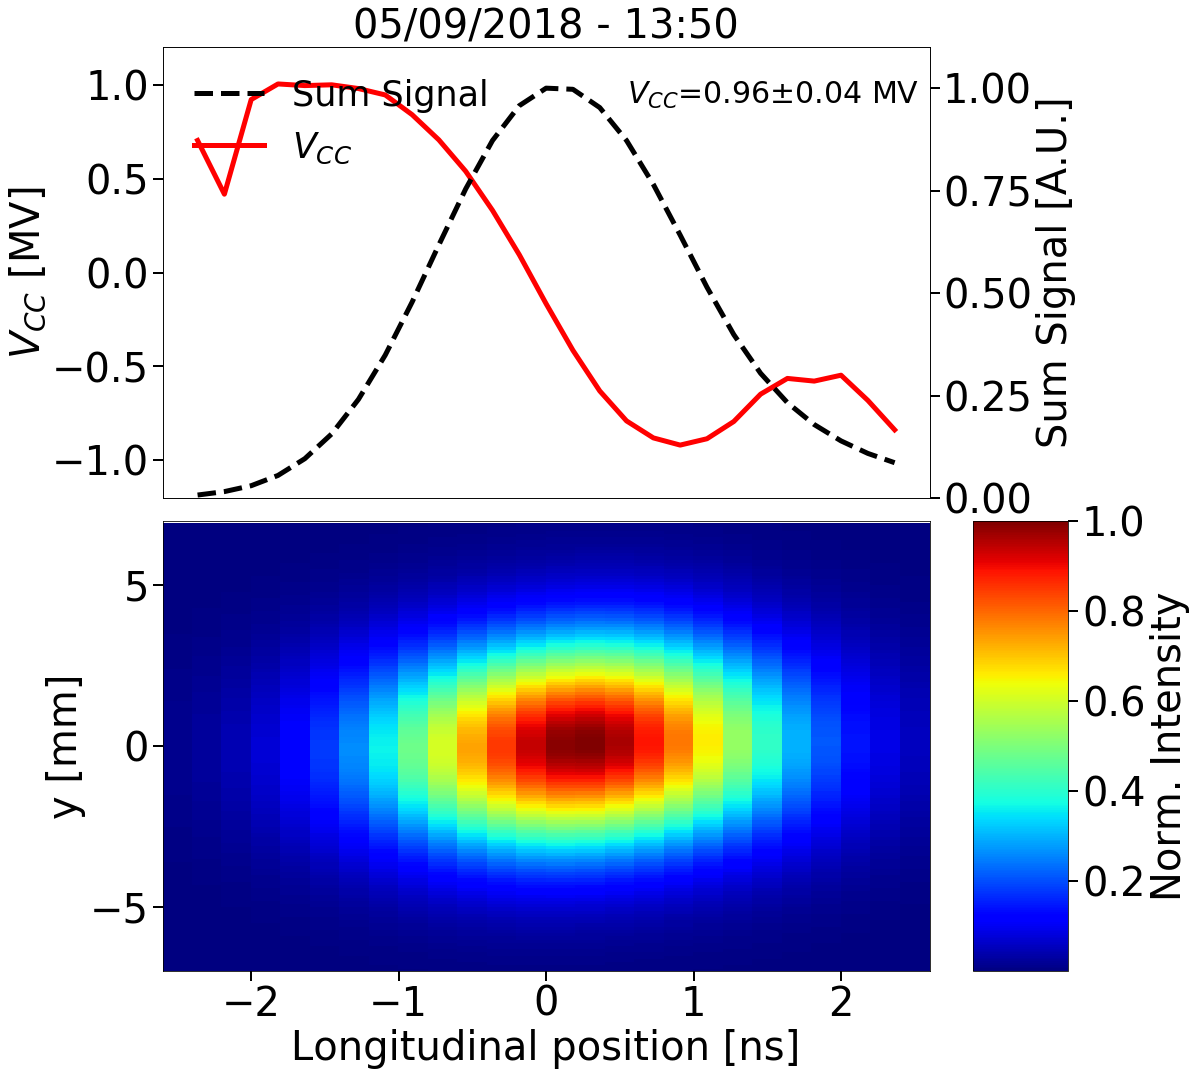
\includegraphics[width=1\textwidth]{images/Ch5/HT_crabVoltage__20180905_135033_crabbing_only.png}
        %\caption{Discrete Fourier transform}
        %\label{fig:signal_and_DFT_example_b}
    \end{subfigure}
    \hfill
     \caption{Measurements of the CC voltage, with the HT monitor (see Section~\ref{subsec:HT_post_process_CC}), before(top-left) and during (top-right) the emittance growth studies. The density plots (bottom) are also shown here to point out that the crabbing is not clearly visible at the energy of 270\,GeV, especially compared to the studies at lower energy (Fig.~\ref{fig:crabbing_reconstruction_HT_monitor}).}
     \label{fig:VCC_MD5_2018} 
\end{figure}

\begin{sloppypar}
The amplitude of the $\CC$ voltage was measured to be 0.75\,$\pm$\,0.37\,MV and 0.96\,$\pm$\,0.04\,MV from the first and the second acquisition respectively. In the following analysis the averaged $\CC$ voltage from the two scans, $V_{CC, \mathrm{avg}}$ = 0.86\,$\pm$\,0.2\,MV , will be used. The uncertainty  $\Delta V_{CC, \mathrm{avg}}$ = 0.2\,MV .. is computed as follows. 

First, the uncertainty in the average, $\Delta V_{CC, \mathrm{avg1}}$, is estimated by (see Appendix ...): 
\end{sloppypar}
\begin{equation}\label{eq:uncertainty_mean_ws}
    \Delta V_{CC, \mathrm{avg1}} = \frac{\mid 0.75 - 0.96 \mid}{2 \sqrt{2}}=0.074\mathrm{\ MV}.
\end{equation}
Then the propagated uncertainty from the measurement errors, 0.37\,MV and 0.04\,MV, is estimated by:
\begin{equation}\label{eq:propagated_uncertainty_ws}
    \Delta V_{CC, \mathrm{avg2}} = \frac{1}{2}\sqrt{ 0.37^2 + 0.04^2} = 0.19\mathrm{\ MV}.
\end{equation}
Considering that $\Delta V_{CC, \mathrm{avg1}}$ and $\Delta V_{CC, \mathrm{avg2}}$ are independent, the combined uncertainty in the average, $\Delta V_{CC, \mathrm{avg}}$, is given by:

\begin{equation}\label{eq:combined_uncertainty_ws}
    \Delta V_{CC, \mathrm{avg}} = \sqrt{\Delta V_{CC, \mathrm{avg1}} ^2 + \Delta V_{CC, \mathrm{avg2}} ^2}=0.2\mathrm{\ MV}.
\end{equation}


\section{Injected RF noise}\label{sec:noise_meas2018}
\begin{sloppypar} % to fix \hbox too wide
 The injected RF noise was a mixture of amplitude and phase noise up to 10\,kHz, overlapping and primarily exciting the first betatron sideband at $\sim 8$\,kHz. The phase noise was always dominant. Figure~\ref{fig:example_PN_and_AN} dsiplays two example measurements of phase (left) and amplitude (right) noise acquired during the experiment with a sepctrum analyzer E5052B~\cite{E5052B_insight}. 
\end{sloppypar} 

 % Loaction for creating the figure: /eos/user/n/natriant/2018/CC_MD_2018_summary/measured_psd
 \begin{figure}[!ht]
    \centering
    \begin{subfigure}[t]{0.45\textwidth}
        \centering
        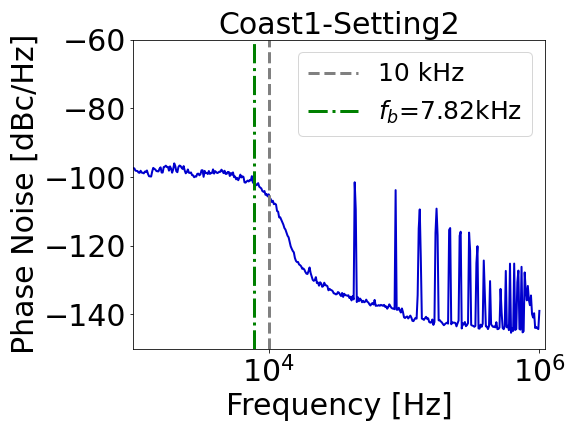
\includegraphics[width=1\textwidth]{images/Ch5/Measured_spectrum_MD5_Coast1-Setting2-PN.csv_no_psd.png}
        %\caption{$y=\sin(2 \pi f t),\ f=50$ Hz}
        %\label{fig:add_label_here}
    \end{subfigure}
    \hfill
    \begin{subfigure}[t]{0.45\textwidth}
        \centering
        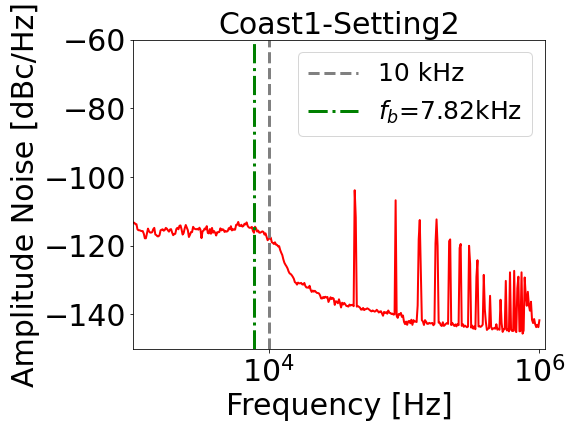
\includegraphics[width=1\textwidth]{images/Ch5/Measured_spectrum_MD5_Coast1-Setting2-AN.csv_no_psd.png}
        %\caption{Discrete Fourier transform}
        %\label{fig:add_label_here}
    \end{subfigure}
    \hfill
     \caption{Example phase (left) and amplitude (right) noise spectra measured with a spectrum analyzer E5052B during the emittance growth studies with CCs in SPS. The noise spread-out up to 10\,kHz (grey dashed line) exciting the first betatron sideband at $\sim$8\,kHz (green dashed line). The spikes at high frequencies correspond to the harmonics of the revolution frequency and are a result of the bunch crossing.} % bunch passage
     \label{fig:example_PN_and_AN}
\end{figure}



\textcolor{red}{The following needs to be refined. I struggled to write it}.
\begin{sloppypar} 
Emittance growth measurements were performed for seven different noise levels, listed in Table~\ref{tab:noise_settings_2018}. The following two points should be highlighted regarding its listings. 
\begin{itemize}
    \item As already discussed in Chapter~\ref{Ch:CC_noise_theory} the noise induced emittance growth depends on the noise power at the beteatron and synchrobetatron sidebands for the phase and amplitude noise respectively (see Eq.~\ref{eq:dey_pn} and Eq.~\ref{eq:dey_an}). Therefore, the noise power values of interest for this thesis are the ones at the first betatron $f_b = 0.18 \times \frev$ = 7.82\,kHz and at the synchrobetatron sidebands at $f_b \pm \Qs \times \frev  = f_b \pm  \sim 220$\,kHz. In the following, it is assumed for simplicity that the noise power at the sidebands mentioned above is the same. Here this assumption is acceptable since the noise power in the measurements is basically constant for all frequencies up to 10\,KHz. 
    \item It is clear from Fig.~\ref{fig:example_PN_and_AN} that the measurements are noisy. In particular random changes in amplitude are observed from point to point within the signal. The values listed in Table~\ref{tab:noise_settings_2018} correspond to the averaged noise values over a frequency range of $\pm$ 500\,Hz around the betatron frequency. The unceratinties show the spread of the values and are defined 
\end{itemize}

\end{sloppypar} 

\begin{table}[!hbt]
	\centering
   \caption{Phase and amplitude noise levels injected in the CC RF system for the emittance growth studies in 2018.}
	\begin{tabu} to \textwidth { X[c,m] X[c,m] X[c,m] X[c,m] }
		&&& \\[-6mm]
		\toprule \toprule
		\multicolumn{2}{l}{} &
		\multicolumn{2}{c}{$\mathbf{10\,\boldsymbol{\log}_{10} \mathcal{L}(f)}$ \textbf{[dBc/Hz]}} \\
		\bottomrule
      \multicolumn{2}{l}{} & 	\multicolumn{1}{c}{\textbf{Phase noise}} & \multicolumn{1}{c}{\textbf{Amplitude noise}} \\
      \midrule
      \multicolumn{2}{l}{Coast1-Setting1}  & \multicolumn{1}{c}{-122.6 $\pm 0.6$} & \multicolumn{1}{c}{-128.1 $\pm$ 0.6} \\
      
      \multicolumn{2}{l}{Coast1-Setting2}  & \multicolumn{1}{c}{-101.4 $\pm$ 0.8} & \multicolumn{1}{c}{-115.2 $\pm$ 0.6} \\

      \multicolumn{2}{l}{Coast2-Setting1}  & \multicolumn{1}{c}{-115.1 $\pm$ 0.8} & \multicolumn{1}{c}{-124.1 $\pm$ 0.5} \\

      \multicolumn{2}{l}{Coast2-Setting2}  & \multicolumn{1}{c}{-111.4 $\pm$ 0.6} & \multicolumn{1}{c}{-115.7 $\pm$ 0.4} \\ 

      \multicolumn{2}{l}{Coast3-Setting1}  & \multicolumn{1}{c}{-110.9 $\pm$ 0.9} & \multicolumn{1}{c}{-116.9 $\pm$ 0.4} \\

      \multicolumn{2}{l}{Coast3-Setting2} & \multicolumn{1}{c}{-106.4 $\pm$ 0.3} & \multicolumn{1}{c}{-112.9 $\pm$ 0.6} \\

      \multicolumn{2}{l}{Coast3-Setting3} & \multicolumn{1}{c}{-101.4 $\pm$ 0.7}  & \multicolumn{1}{c}{-106.9 $\pm$ 0.5} \\
      \arrayrulecolor{black}\bottomrule
 
	\end{tabu}
   \label{tab:noise_settings_2018}
\end{table}



\begin{sloppypar} % to fix \hbox too wide
This spectrum analyzer provides a single sideband measurement (SSB), which is expressed as $10\log_{10}\mathcal{L}(f)$\,[dBc/Hz]. Its relation with the power spectral densities (PSDs) introduced in Eq.~\eqref{eq:dey_an} and Eq.~\eqref{eq:dey_pn} are given by $S_\Delta = 2\mathcal{L}(f)$~\cite{IEEE:4797525}, with $S_{\Delta A}$ in 1/Hz and $S_{\Delta\phi}$ in rad$^2$/Hz. A detailed discussion on the noise power measurements and their relation to the mathimatical defintion of the PSD is given in Chapter [tba].

As already mentioned above, the injected noise was a combination of both phase and amplitude noise. Therefore, in order to make a meaningful comparison between the different noise levels the concept of effective phase noise is introduced. This is the phase noise level that would lead to
the same emittance growth as that from both phase and
amplitude noise. The noise levels mentioned in this chapter correspond to the calculated effective phase noise.
% should I slightly change this paragraph? Too much copy paste from IPAC or it's ok?
\end{sloppypar} 



\section{Emittance growth measurements}\label{sec:EmitGrowth_measurements}

An overview of the bunch by bunch emittance growth measurments is shown in Fig ... for both horizontal (top) and vertical (bottom) plane. The four different colors (blue, orange, green, red) correspond to the four different bunches. The three "coasts" are distinguishable with the black dashed vertical lines. For each "coast" a new beam was injected with the same targeted initial conditions. The different levels of injected noise are also displayed in the plot (bottom) while the moments at which the noise level changed are shown with the grey dashed vertical lines. These noise levels are the average of the effective phase noise over the four bunches (due to different bunch lengths.)


What should be observed is the following: ...

% Figures for emit growth evolution MD 2018: SWAN_projects/CC_MDs_2018/myAnalysis_2020/for_thesis/average_MD5_overview_5Sep2018_emitBU_PlotOverview_Vertical_OpenRatesFromPickle_for_thesis.ipynb


MD emittance growth overview. 
    - average from IN and OUT. As mentioned in CH4. vs time and vs noise level for all bunches. Not yet comparison with the theory. Probably you need to re-run this to make correctly the error propagation. 
    - 1 noise point was excluded
 


\section{Bunch length measurements}\label{sec:bunch_length_measurements_2018}
    - bunch length and longitudinal profiles and relative position from the wall current monitor.  unstable bunches.
    - bunch 2-3-4 longutidinally unstable.
 
\section{Intensity measurements}\label{sec:intensity_measurements_2018}
No losses. Maybe not seperate chapter?
I should also mention in Ch4 how the emittance is measured from the ABWLM.

\section{Comparison of measured emittance growth with the theory}\label{sec:meas_2018_vs_theory}

Comparison of bunch 1 with theory. Discrepancy of a factor 4.


 \section{Conclusions and outlook}\label{sec:MD2018_summary}



 test line for new branch.